% Calibration-free discrimination of unresolved sources -- draft for Physical Review A (Regular Article), REVTeX 4.2.
% Rules: STYLE_AND_VENUE.md. Every number traces to results/*.json via research/CLAIMS_LEDGER.md (S15-S17d).
% Tables: gen_tables.py. Figures: gen_figures.py. Author and affiliation data from submission/sn-article.tex.
\documentclass[reprint,pra,aps,amsmath,amssymb,superscriptaddress,nofootinbib]{revtex4-2}
\usepackage{graphicx}
\usepackage{bm}
\usepackage{xcolor}
\usepackage[hidelinks]{hyperref}
\newcommand{\todo}[1]{\textcolor{red}{[TODO: #1]}}
\newcommand{\ket}[1]{|#1\rangle}
\newcommand{\bra}[1]{\langle #1|}
\newcommand{\sym}{\mathrm{Sym}}

\begin{document}

\title{Calibration-free discrimination of unresolved sources with symmetric multiphoton measurements}

\author{Prathamesh Balasaheb Kadam}
\email{prathamesh.kadam@aissmsioit.org}
\author{Prajwal S. Gaikwad}
\author{Shreyas Subhash Raut}
\author{Tejas Uttam Shitole}
\affiliation{Department of Artificial Intelligence and Data Science, AISSMS Institute of Information Technology,
Pune, India}

\date{\today}

\begin{abstract}
A single star and a close binary can be told apart at the quantum limit by sorting photons into Hermite-Gauss
modes, but only if the sorter is aligned with the centroid of the source. We compute exact error exponents for
this test when the pointing is unknown and must be learned from photons. Measure-first learners estimate the
centroid by direct imaging of calibration or target photons and then sort modes. They retain a fraction of the
known-pointing quantum Chernoff exponent that depends only on the calibration budget: 17\%--20\% without
calibration, and 33\%, 63\% and 69\% with 1, 100 and 1000 calibration photons per target photon, at every
separation. The residual pointing error turns the zero-background test into a background-limited one, and no
single-photon receiver that we optimized escapes this limit. Projecting $k$ stored target photons onto the
symmetric subspace of their transverse states instead has zero background for every pointing offset and every
static mode crosstalk. It attains a fraction $(k-1)/k$ of the quantum limit without any calibration. Groups of four
photons already outperform 1000 calibration photons per target photon, and the gain in error exponent is 1.6 to
5.7. With a single target photon, joint learning keeps a constant 18\% advantage in excess risk over measure-first
learning, through an interference port that is dark for every pointing. Invariance under translations alone gains
at most 1\% over the two-photon Hong-Ou-Mandel test.
\end{abstract}

\maketitle

% =====================================================================================================
\section{Introduction}

Telling a single star from a close binary below the Rayleigh limit is a hypothesis test. Its quantum limit is
reached by sorting the light into Hermite-Gauss (HG) modes centered on the source \cite{Tsang2016,Lu2018,Grace2022}.
The error exponent of direct imaging vanishes as the fourth power of the separation, while the quantum exponent
vanishes only as its square. The origin of the advantage is simple: a single source sends every photon into the
fundamental mode, so a photon in any other mode signals a second source.

The same zero-background structure makes the advantage fragile. Crosstalk or misalignment of the sorter leaks
single-source photons into the signal ports. The simple test then fails, and the optimal test recovers the quantum
exponent only logarithmically as the leak vanishes \cite{Schlichtholz2023}. A fixed offset removes the support
mismatch on which the ideal test relies \cite{Kariya2026}. Measurements tailored to a known offset reduce the loss
but do not remove it \cite{deAlmeida2021}. Existing analyses assume that the centroid is known \cite{Zanforlin2022},
or treat the offset as fixed. In practice the pointing has to be learned from photons, either from calibration
exposures or from the target itself \cite{Grace2020}.

This makes the test a problem of learning from quantum data \cite{Sentis2012,Guta2010,Sentis2015}. A measure-first
learner detects each photon and processes the outcomes classically. A coherent learner can store photons and
measure them jointly. For estimation, collective measurements that exploit permutation symmetry are robust to
misalignment \cite{deAlmeida2025}, and two-photon interference beats the Rayleigh limit
\cite{Parniak2018,Muratore2024}. For discrimination with a learned pointing, neither the cost of calibration nor a
calibration-free alternative has been quantified.

We compute exact error exponents for both kinds of learner; all predictions were pre-registered
(Appendix~\ref{app:prereg}). There are three main results.
\begin{enumerate}
\item Measure-first learners stay background-limited for any finite calibration budget. They retain a
  separation-independent fraction of the known-pointing exponent, from 0.17--0.20 without calibration to 0.69 with
  1000 calibration photons per target photon (Sec.~\ref{sec:classical}).
\item Symmetric projection of stored photons removes the calibration problem. It has zero background for any
  pointing and any static crosstalk, attains $(k-1)/k$ of the quantum limit, and gives a 1.6- to 5.7-fold larger
  exponent (Sec.~\ref{sec:quantum}).
\item With one target photon, joint learning keeps a constant 18\% advantage through a dark interference port
  (Sec.~\ref{sec:single}).
\end{enumerate}
Section~\ref{sec:invariance} shows that invariance under translations alone gains at most 1\% over the
Hong-Ou-Mandel (HOM) test, so permutation symmetry is the right invariance. Section~\ref{sec:discussion} discusses
implementations and limitations.

% =====================================================================================================
\section{One-versus-two testing with an unknown pointing}
\label{sec:setting}

We work in one transverse dimension, with a Gaussian point-spread function of unit width. In the weak-source
regime a photon from a point source at $x$ is in the state $\ket{\psi_x}$, with amplitude
$\psi(y-x)\propto e^{-(y-x)^2/4}$. In the HG basis these are coherent states of an oscillator,
$\langle\mathrm{HG}_n|\psi_x\rangle=e^{-a^2/2}a^n/\sqrt{n!}$ with $a=x/2$, and their overlaps are
$\langle\psi_x|\psi_y\rangle=e^{-(x-y)^2/8}$.

Under $H_0$ every photon is in $\rho_0(\theta)=\ket{\psi_\theta}\bra{\psi_\theta}$. Under $H_1$ it is in
$\rho_1(\theta)=\tfrac12(\ket{\psi_{\theta+d/2}}\bra{\psi_{\theta+d/2}}+\ket{\psi_{\theta-d/2}}\bra{\psi_{\theta-d/2}})$,
an equal-brightness binary of separation $d$ with the same centroid. We write $a_0=d/4$. The pointing offset
$\theta$ is unknown and static. The learner receives $N$ target photons from one hypothesis (equal priors) and,
optionally, $\kappa N$ labeled calibration photons from a known single source at the same pointing. Performance is
measured by the error exponent per target photon, $E=\lim_{N\to\infty}-N^{-1}\ln P_{\rm err}$.

If $\theta$ is known, the quantum Chernoff exponent \cite{Audenaert2007,Nussbaum2009} for the pure $\rho_0$ is
$\xi_Q=-\ln\bra{\psi_\theta}\rho_1\ket{\psi_\theta}=a_0^2$ exactly. It is attained by the null test
$\{\ket{\psi_\theta}\bra{\psi_\theta},1-\ket{\psi_\theta}\bra{\psi_\theta}\}$, which never clicks under $H_0$ and
clicks with probability $1-e^{-a_0^2}$ under $H_1$. We report all exponents as fractions of $a_0^2$.

% =====================================================================================================
\section{Measure-first learners stay background-limited for any calibration budget}
\label{sec:classical}

A measure-first learner estimates the centroid and then measures the remaining target photons at the estimate.
Direct imaging attains the quantum Fisher information for the centroid. If the $\kappa N$ calibration photons and a
fraction $f$ of the target photons are imaged, the residual offset $t=\theta-\hat\theta$ has the large-deviation rate
$g(t)=(\kappa+f)t^2/2$ per target photon. The other $(1-f)N$ target photons enter a single-photon receiver centered
at $\hat\theta$, with outcome probabilities $p_{cj}(t)$ under $H_c$. The Bayes error exponent is
(Appendix~\ref{app:ld})
\begin{multline}
E(\kappa,f)=\min_{t_0,t_1}\max_{0\le s\le1}\Big[s\,g(t_0)+(1-s)\,g(t_1)\\
-(1-f)\ln\sum_j p_{0j}(t_0)^s\,p_{1j}(t_1)^{1-s}\Big],
\label{eq:ld}
\end{multline}
which we maximize over $f$. Here $t_0$ and $t_1$ are the worst-case offsets under the two hypotheses. We evaluate
Eq.~\eqref{eq:ld} for two receivers:
\begin{itemize}
\item HG sorting, with outputs $\mathrm{HG}_0,\dots,\mathrm{HG}_5$ and a rest port;
\item a real orthogonal six-mode receiver, optimized numerically to maximize Eq.~\eqref{eq:ld}.
\end{itemize}
The optimized receiver mixes modes of opposite parity, so its worst case has to be searched over offsets of both
signs.

\begin{table*}[t]
\caption{Error exponents per target photon in units of the known-pointing quantum limit $a_0^2$ ($a_0=0.1$).
Measure-first learners combine direct-imaging centroiding, with $\kappa$ calibration photons per target photon and a
fraction $f^\ast$ of the target photons, with HG sorting or with an optimized six-mode receiver. ``Coherent
references'' projects each target photon jointly with $\kappa$ calibration photons onto their symmetric subspace.
The measure-first values are identical to three digits for $a_0=0.05$ and 0.2. Generated from
\texttt{results/qx3e/qx3e.json}.}
\label{tab:exponents}
% generated by gen_tables.py from results JSON - do not edit by hand
\begin{ruledtabular}
\begin{tabular}{rcccc}
$\kappa$ & measure-first (SPADE) & $f^\ast$ & measure-first (learned) & coherent references \\
\colrule
0 & 0.174 & 0.41 & 0.203 & -- \\
0.1 & 0.191 & 0.29 & -- & -- \\
0.3 & 0.226 & 0.17 & -- & -- \\
1 & 0.334 & 0.00 & 0.334 & 0.499 \\
3 & 0.439 & 0.00 & -- & 0.749 \\
10 & 0.525 & 0.00 & 0.525 & 0.909 \\
30 & 0.582 & 0.00 & -- & 0.968 \\
100 & 0.629 & 0.00 & 0.629 & 0.990 \\
1000 & 0.691 & 0.00 & -- & -- \\
\colrule
\multicolumn{5}{l}{Symmetric projection of $k$ stored target photons, no calibration:} \\
\multicolumn{5}{l}{$k=2$: 0.493, $k=3$: 0.660, $k=4$: 0.744, $k=8$: 0.869, $k=16$: 0.932; $k\to\infty$: 0.9950} \\
\end{tabular}
\end{ruledtabular}

\end{table*}

Table~\ref{tab:exponents} and Fig.~\ref{fig:exponents} show the result.
\begin{itemize}
\item \emph{No calibration.} HG sorting retains 17.4\% of the quantum limit, spending $f^\ast=0.41$ of the target
  photons on centroiding. The optimized receiver retains 20.3\%, because it extracts the centroid and the binary
  signal from the same photons.
\item \emph{With calibration.} Centroiding on the target stops paying ($f^\ast=0$ for $\kappa\ge1$), and the
  optimized receiver coincides with HG sorting.
\item \emph{Slow growth.} The retained fraction $F(\kappa)$ is 33\% at $\kappa=1$, 52\% at 10, 63\% at 100 and 69\%
  at 1000; an exploratory point gives 82\% at $\kappa=10^8$.
\end{itemize}
$F(\kappa)$ is the same for $a_0=0.05$, 0.1 and 0.2. The worst case pairs an offset single source with a centered
binary, both Poissonian in the mode basis, so the exponent is homogeneous in $a_0^2$ (Appendix~\ref{app:ld}).

\begin{figure}[t]
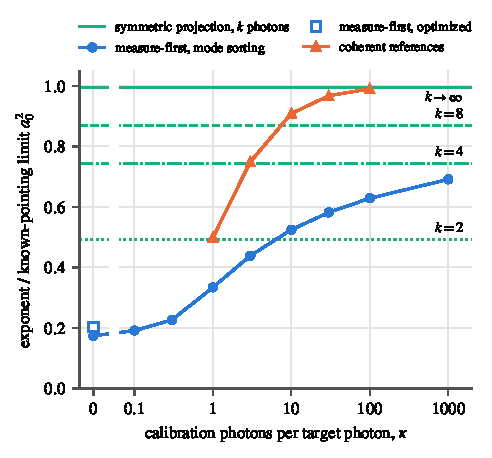
\includegraphics[width=\columnwidth]{figures/fig1_exponents.pdf}
\caption{Error exponent per target photon in units of the known-pointing limit $a_0^2$ ($a_0=0.1$).
Circles: measure-first learning (direct-imaging centroiding, HG sorting) with $\kappa$ calibration photons per
target photon; $\kappa=0$ is shown left of the axis break.
Open square: optimized single-photon receiver at $\kappa=0$.
Triangles: each target photon projected jointly with $\kappa$ calibration photons onto their symmetric subspace.
Horizontal lines: symmetric projection of groups of $k$ stored target photons, without calibration.}
\label{fig:exponents}
\end{figure}

The mechanism is a background.
\begin{itemize}
\item A residual offset $t_0$ sends single-source photons into $\mathrm{HG}_1$ at the rate $u\,a_0^2$, with
  $u=t_0^2/4a_0^2$, while the binary sends photons there at the rate $a_0^2$.
\item The Chernoff exponent between these two Poisson rates is $a_0^2h(u)$, with $h(u)=\max_s[su+1-s-u^s]$. It
  recovers only as $1-[\ln\ln(1/u)-1]/\ln(1/u)$, the law found for crosstalk in Ref.~\cite{Schlichtholz2023}.
\item Balancing the cost $2(\kappa+f)u$ of a larger offset against this loss gives
  $E/a_0^2\simeq\min_u[2(\kappa+f)u+(1-f)h(u)]$, which reproduces $F(\kappa)$.
\end{itemize}
Every port that carries a second-order signal from the binary also carries a second-order background from the
offset. Each target photon provides at most unit centroid Fisher information. No single-photon receiver therefore
escapes the trade-off.

For finite photon numbers we computed the exact Bayes error of three-outcome HG sorting, summing the multinomial
distribution over the normal residual offset. At $a_0=0.1$ and $N=8000$ it is $1.6\times10^{-13}$ for $\kappa=1$ and
$3.3\times10^{-20}$ for $\kappa=10$. The local exponents at $N=4000$--8000 agree with Eq.~\eqref{eq:ld} to within 3\%
(Fig.~\ref{fig:finiteN}).

\begin{figure}[t]
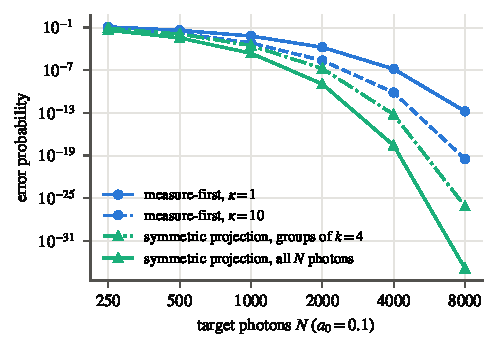
\includegraphics[width=\columnwidth]{figures/fig2_finite_n.pdf}
\caption{Exact error probabilities versus the number of target photons $N$ ($a_0=0.1$).
Circles: measure-first learning with $\kappa=1$ and 10.
Triangles: symmetric projection in groups of $k=4$ and of all $N$ photons, $P_{\rm err}=\tfrac12h_k^{N/k}$.}
\label{fig:finiteN}
\end{figure}

\emph{Takeaway.} Learning the pointing and then measuring cannot recover the quantum advantage. Even 100 calibration
photons per target photon leave the learner at 63\% of the known-pointing exponent, at every separation.

% =====================================================================================================
\section{Symmetric projection removes the calibration problem}
\label{sec:quantum}

A coherent learner can avoid learning $\theta$. It stores $k$ target photons in distinguishable time bins and
projects their joint transverse state onto the symmetric subspace $\sym^k$.
\begin{itemize}
\item \emph{Under $H_0$} the $k$ photons share the pure state $\ket{\psi_\theta}$, so the projection never fails. This
  holds for every $\theta$ and under any static crosstalk $U$, because $U^{\otimes k}$ preserves $\sym^k$.
\item \emph{Under $H_1$} the photons are independent copies of $\rho_1(\theta)$, whose eigenvalues
  $\lambda_\pm=\tfrac12(1\pm e^{-2a_0^2})$ do not depend on $\theta$. The projection succeeds with probability
  $h_k(\lambda_+,\lambda_-)=\sum_{j=0}^k\lambda_+^j\lambda_-^{k-j}$ (Appendix~\ref{app:sym}).
\end{itemize}
Declaring two sources as soon as one group fails gives $P_{\rm err}=\tfrac12h_k^{N/k}$, hence
\begin{gather}
E_k=-\tfrac1k\ln h_k(\lambda_+,\lambda_-)\simeq\tfrac{k-1}{k}\,a_0^2,\label{eq:schur}\\
E_\infty=-\ln\tfrac{1+e^{-2a_0^2}}{2}=a_0^2-\tfrac{a_0^4}{2}+\dots\nonumber
\end{gather}
For $k=2$ this is the HOM test.

The exponents are $E_2=0.49$, $E_4=0.74$ and $E_8=0.87$, and $E_\infty=0.9988$, 0.9950 and 0.9800 at $a_0=0.05$, 0.1
and 0.2, all in units of $a_0^2$ (Table~\ref{tab:exponents}, Fig.~\ref{fig:exponents}).
\begin{itemize}
\item \emph{Group sizes.} HOM pairs beat measure-first learning up to about three calibration photons per target
  photon, triples up to about 100, groups of four at 1000, and groups of eight even at the exploratory
  $\kappa=10^8$.
\item \emph{Gain.} Large groups exceed the best measure-first exponent by a factor 4.9--5.7 without calibration,
  3.0 at $\kappa=1$, 1.9 at $\kappa=10$ and 1.6 at $\kappa=100$.
\item \emph{Finite $N$.} At $N=8000$ and $a_0=0.1$ the error is about $10^{-35}$, against $1.6\times10^{-13}$ for
  measure-first learning with $\kappa=1$.
\end{itemize}

Calibration photons can also be used coherently. Projecting each target photon together with $\kappa$ fresh
calibration photons fails under $H_1$ with probability $\kappa(1-e^{-a_0^2})/(\kappa+1)$ and never under $H_0$, so
$E\simeq a_0^2\kappa/(\kappa+1)$. For the same calibration budget this beats measuring the calibration photons by a
factor 1.5 ($\kappa=1$), 1.7 ($\kappa=10$) and 1.6 ($\kappa=100$).

\emph{Takeaway.} A measurement that is blind to the pointing by symmetry recovers, without calibration, the advantage
that measure-first learners lose to calibration. Four stored photons beat 1000 calibration photons per target
photon.

% =====================================================================================================
\section{With one target photon, joint learning keeps a constant advantage}
\label{sec:single}

The single-photon version of the problem connects to quantum learning theory \cite{Sentis2012,Guta2010,Sentis2015}.
\begin{itemize}
\item \emph{Setting.} Let $\theta\sim\mathcal N(0,\tau^2)$. The learner receives $n$ calibration photons and one
  target photon. Performance is the excess Bayes risk over the known-pointing error; the known-pointing advantage
  is $\tfrac12-P_{\rm known}=0.678\,a_0^2$.
\item \emph{Exact reduction.} The calibration photons are unitarily equivalent to one collective coherent state
  $\ket{\sqrt n\,\theta/2}$ (Appendix~\ref{app:collective}). This makes the joint Helstrom optimum exactly
  computable.
\end{itemize}

Results ($a_0\in\{0.05,0.1,0.2\}$, $\tau\in\{0.2,0.5\}$, $n\le128$; exploratory up to 1024):
\begin{itemize}
\item \emph{Constant gap.} Measure-first learning (direct imaging of the calibration photons, then the Bayes test)
  has an excess risk 1.16--1.19 times that of the joint optimum for $n\ge16$. The factor tends to 1.184 and is
  independent of $a_0$ to within 1\% [Fig.~\ref{fig:single}(a)].
\item \emph{Plug-in is nearly optimal.} Estimating $\theta$ and applying the known-pointing Helstrom measurement costs
  at most 0.8\% extra for $n\ge16$.
\item \emph{Sign-blind calibration is useless.} HG counting of the calibration photons on the nominal axis recovers
  95.6\% of the known-pointing advantage at $n=128$, against 95.5\% with no calibration ($\tau=0.2$). Its posterior
  is symmetric about the axis, so its average spread about the axis equals the prior spread
  [Fig.~\ref{fig:single}(b)].
\end{itemize}

\begin{figure}[t]
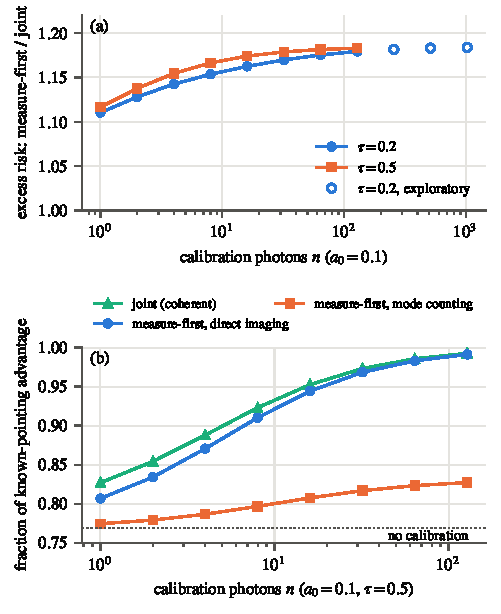
\includegraphics[width=\columnwidth]{figures/fig3_single_photon.pdf}
\caption{One target photon.
(a) Excess risk of measure-first learning divided by that of the joint optimum ($a_0=0.1$; $a_0=0.05$ and 0.2 agree
within 1\%). Open circles: exploratory, not pre-registered.
(b) Fraction of the known-pointing advantage recovered ($\tau=0.5$). Dotted: no calibration.}
\label{fig:single}
\end{figure}

The mechanism is an interference port. Interfering the target photon with the collective calibration mode, with
amplitude weights $\sqrt n:1$, gives an output that is in vacuum under $H_0$ for every $\theta$. Under $H_1$ that
output carries a $\theta$-independent binary with $a_0^2$ reduced by $n/(n+1)$.
\begin{itemize}
\item The joint learner therefore pays for the pointing uncertainty as a slightly smaller separation, with excess
  risk $\simeq0.678\,a_0^2/(n+1)$. The dark port alone comes within 3\% of the optimum at $n=128$ ($\tau=0.5$).
\item The measure-first learner pays for it as an incoherent jitter, with excess risk
  $\simeq c\times0.678\,a_0^2/(n+1/\tau^2)$, where $c\to1.18$.
\end{itemize}
A constant asymptotic gap between joint and Gaussian measure-first learning is known for coherent-state templates
\cite{Sentis2015}. Here it appears in the imaging problem, with a closed-form mechanism.

\emph{Takeaway.} With one target photon the coherent advantage is a modest 18\%. With many photons the same dark-port
structure removes the background, and the advantage becomes decisive (Sec.~\ref{sec:quantum}).

% =====================================================================================================
\section{Translation invariance alone buys almost nothing}
\label{sec:invariance}

Symmetric projection is invariant under every common mode transformation, whereas the physical nuisance is only a
translation. A measurement invariant under translations alone might therefore extract more information. We tested
this for two photons sharing a slow common jitter of width $s_j$ and a static random crosstalk on the first 13 HG
modes.
\begin{itemize}
\item \emph{Only the relative coordinate is usable.} A translation-invariant measurement is block diagonal in the
  total momentum of the pair, and the total momentum is uninformative.
\item \emph{Its optimum.} The best such measurement refines HOM by projecting the relative coordinate onto its
  fundamental mode. It clicks under $H_1$ with probability $(1-e^{-d^2/8})/2$, against $(1-e^{-d^2/4})/4$ for HOM.
\item \emph{The gain.} The relative gain is $2/(1+e^{-d^2/8})-1\simeq d^2/16$: 0.06\%, 0.25\% and 1.0\% at $d=0.1$,
  0.2 and 0.4, independent of the jitter (Table~\ref{tab:invariance}).
\item \emph{Fragility.} The coarse version of the test leaks $\approx25\epsilon^2$ under $H_0$ for our crosstalk
  model, and falls below HOM already at $\epsilon=10^{-4}$.
\item \emph{Learned measurements.} A two-photon measurement trained over a box of jitter and crosstalk values beats
  HOM by 0.2\%--1.0\% in the worst case; the best possible pair measurement beats HOM by 0.4\%--1.5\% there. The
  learned measurement is never below HOM, and is 1.5--1.7 times better than HOM at zero jitter.
\end{itemize}

\begin{table*}[t]
\caption{Two-photon exponents relative to HOM. $E_{\rm T}$: optimal translation-invariant measurement (any
jitter). $E_{\rm pair}$: optimal pair measurement at jitter $s_j$. $\epsilon^\ast$: crosstalk at which the coarse
translation-invariant test falls below HOM ($s_j=0.4$). Generated from \texttt{results/qx2/qx2.json}.}
\label{tab:invariance}
% generated by gen_tables.py from results JSON - do not edit by hand
\begin{ruledtabular}
\begin{tabular}{lcccc}
$d/\sigma$ & $E_{\rm T}/E_{\rm HOM}$ & $E_{\rm pair}/E_{\rm HOM}$ ($s_j=0$) & $E_{\rm pair}/E_{\rm HOM}$ ($s_j=0.8$) & $\epsilon^\ast$ \\
\colrule
0.1 & 1.0006 & 2.002 & 1.0009 & 1e-04 \\
0.2 & 1.0025 & 2.008 & 1.0037 & 1e-04 \\
0.4 & 1.0100 & 2.030 & 1.0149 & 1e-04 \\
1 & 1.0643 & 2.197 & 1.0967 & 3e-03 \\
\end{tabular}
\end{ruledtabular}

\end{table*}

\emph{Takeaway.} Below the Rayleigh limit, full permutation symmetry costs almost nothing relative to the symmetry of
the physical nuisance, and it buys immunity to crosstalk.

% =====================================================================================================
\section{Discussion}
\label{sec:discussion}

\emph{Implementation.}
\begin{itemize}
\item The symmetric projection requires $k$ photons held in a quantum memory and released together. Only the photons
  within one group need to share the pointing, so drift between groups is harmless.
\item For $k=2$ it is the HOM test, a beam splitter followed by coincidence detection.
\item For larger $k$ it is weak Schur sampling of the transverse state. Implementations with atomic memories,
  multiport devices and linear optics have been proposed for estimation \cite{deAlmeida2025}, and multiport
  interferometers resolve distinguishability classes of photons \cite{Stanisic2018}.
\item Imperfect storage reintroduces a background. In a two-photon calculation with the same model (data in the
  repository), a random mode mismatch of strength $\epsilon$ between the two memories gives an $H_0$ background
  $\approx3.8\epsilon^2$ for our mismatch model. A differential pointing jitter $s_d$ between the stored photons gives
  $[1-(1+s_d^2)^{-1/2}]/2\approx s_d^2/4$. Both must stay below the binary signal $\approx a_0^2$.
\end{itemize}

\emph{Limitations.}
\begin{itemize}
\item One transverse dimension, an equal-brightness binary, a Gaussian point-spread function and ideal detectors.
\item Asymptotic exponents, with a finite-$N$ check at one separation.
\item The measure-first family consists of direct-imaging centroiding followed by one fixed single-photon receiver.
  Adaptive multi-stage receivers are not excluded, although each target photon carries at most unit centroid
  information.
\end{itemize}
Unequal brightness (the exoplanet case), two-dimensional pointing and slow drift within a group remain open.

The broader lesson is that a measurement invariant under a nuisance replaces learning the nuisance. For sub-Rayleigh
discrimination the right invariance is the permutation symmetry of stored photons. Its cost is a quantum memory, not
more light.

% =====================================================================================================
\begin{acknowledgments}
We thank the maintainers of NumPy, SciPy, PyTorch and Matplotlib, on which all numerical work in this paper
depends. This work received no external funding.

\emph{Use of AI tools.}
\begin{itemize}
\item \emph{Tools.} This work made substantive use of Claude Opus 5.5 (Anthropic; model identifier
  \texttt{claude-opus-5-5}), run through Claude Code. Claude Sonnet 5.5 sub-agents were used for literature
  searches.
\item \emph{What it did, under the authors' direction:}
  \begin{itemize}
  \item derived the analytic results;
  \item wrote and ran the simulation code;
  \item carried out the literature searches and novelty checks;
  \item drafted the manuscript.
  \end{itemize}
\item \emph{Direction and verification.} P.~B.~Kadam directed all of the work: he chose the research questions,
  approved each stage, and verified and checked all of the calculations reported here by hand.
\item \emph{Controls.}
  \begin{itemize}
  \item Every prediction was committed to a version-controlled pre-registration file before the code that tested
    it existed.
  \item All results were computed on the authors' hardware, and every figure and table is regenerated by scripts
    from version-controlled result files.
  \end{itemize}
\end{itemize}
\end{acknowledgments}

\emph{Data availability.} The code and numerical results that support the findings of this article are openly
available \cite{QKrepo}.

% =====================================================================================================
\appendix
% Appendices of the calibration-free discrimination paper (input by main.tex after \appendix).

\section{Large-deviation exponent of measure-first learners}
\label{app:ld}

Each imaged photon has a position distributed normally around $\theta$ with unit variance. With a flat prior on
$\theta$, the residual offset $t$ is then normal with variance $[(\kappa+f)N]^{-1}$. (Under $H_1$ the true variance
of target photons is $1+d^2/4$, so this slightly favors the measure-first learner.) The remaining $M=(1-f)N$ target
photons give counts $\bm m$, with probability
\begin{equation}
P_c(\bm m)=\int dt\,\phi_N(t)\,\mathrm{Mult}\big(\bm m;M,p_c(t)\big)
\end{equation}
under $H_c$. Write $x=\bm m/M$ for the empirical distribution. Sanov's theorem and Laplace's method give
\begin{equation}
-N^{-1}\ln P_c\to\min_t[g(t)+(1-f)D(x\|p_c(t))].
\end{equation}
The Bayes error is dominated by the most likely confusable $x$, so
$E=\min_{t_0,t_1}\min_x\max_c[g(t_c)+(1-f)D(x\|p_c(t_c))]$. Writing the maximum as a maximum over convex weights
$s$, exchanging the minimum and maximum (Sion's theorem), and using
$\min_x[sD(x\|p)+(1-s)D(x\|q)]=-\ln\sum_jp_j^sq_j^{1-s}$ gives Eq.~\eqref{eq:ld}.

\emph{Separation independence.} Under HG sorting a single source at offset $t_0$ gives
$\mathrm{Poisson}(t_0^2/4)$ mode statistics. A centered binary gives $\mathrm{Poisson}(a_0^2)$, because both emitters
have $a^2=a_0^2$. For this pair the sum in Eq.~\eqref{eq:ld} is
$\exp[-st_0^2/4-(1-s)a_0^2+(t_0^2/4)^sa_0^{2(1-s)}]$, and $g(t_0)=2(\kappa+f)a_0^2u$ with $u=t_0^2/4a_0^2$. Every term
is proportional to $a_0^2$, so $E/a_0^2$ depends on $\kappa$ alone whenever $t_1=0$. The numerically found worst
case has $|t_1|<10^{-8}d$ at every $\kappa$ and $a_0$.

\emph{Numerical details.} Zero port probabilities restrict the sum to the common support, and the endpoints
$s\to0^+$ and $1^-$ are taken as one-sided limits. HG sorting satisfies $p_c(t)=p_c(-t)$, so offsets $t\ge0$
suffice. Receivers that mix modes of opposite parity need offsets of both signs.

\section{Symmetric-projection probabilities}
\label{app:sym}

Let $\rho=\sum_i\lambda_i\ket{e_i}\bra{e_i}$. The symmetrized occupation-number states $\ket{\bm m}$ ($\sum_im_i=k$)
built from the $e_i$ form an orthonormal basis of $\sym^k$, and $\rho^{\otimes k}$ acts on $\ket{\bm m}$ with
eigenvalue $\prod_i\lambda_i^{m_i}$. Hence $\mathrm{Tr}[\Pi_{\sym^k}\rho^{\otimes k}]=h_k(\lambda)$, the complete
homogeneous symmetric polynomial.
\begin{itemize}
\item \emph{Eigenvalues.} For $\rho_1=\tfrac12(\ket\alpha\bra\alpha+\ket\beta\bra\beta)$ with
  $|\langle\alpha|\beta\rangle|=e^{-d^2/8}=e^{-2a_0^2}$, the eigenvalues are $\lambda_\pm=\tfrac12(1\pm e^{-2a_0^2})$.
  They are independent of $\theta$ and of any common unitary.
\item \emph{Invariance under $H_0$.} $(U\ket{\psi_\theta})^{\otimes k}\in\sym^k$ for every $\theta$ and $U$.
\item \emph{Exponent.} Expanding $h_k=\lambda_+^k\sum_{j=0}^k(\lambda_-/\lambda_+)^j$ gives
  $E_k\simeq(1-1/k)\lambda_-\simeq\tfrac{k-1}{k}a_0^2$. As $k\to\infty$, $E_k\to-\ln\lambda_+<a_0^2$.
\end{itemize}

\emph{Projection with calibration photons.} Write $\ket\phi=c\ket\psi+s\ket{\psi^\perp}$; the component
$\ket\psi^{\otimes n}\ket{\psi^\perp}$ has squared norm $1/(n+1)$ after symmetrization. Hence
\begin{equation}
\mathrm{Tr}[\Pi_{\sym^{n+1}}(\ket\psi\bra\psi^{\otimes n}\otimes\ket\phi\bra\phi)]=(1+n|c|^2)/(n+1).
\end{equation}
With $|c|^2=|\langle\psi_\theta|\psi_{\theta\pm d/2}\rangle|^2=e^{-a_0^2}$, the projection fails under $H_1$ with
probability $\kappa(1-e^{-a_0^2})/(\kappa+1)$.

\section{Collective-mode reduction and the dark port}
\label{app:collective}

\emph{Reduction.} A photon from a point source at $x$ is in the coherent state $\ket{x/2}$ of the HG oscillator. The
$n$-mode discrete Fourier transform of the photons' ladder operators maps $\ket\alpha^{\otimes n}$ to
$\ket{\sqrt n\,\alpha}\otimes\ket0^{\otimes(n-1)}$, so the joint states are
$\Omega_c=\int d\pi(\theta)\,\ket{\sqrt n\theta/2}\bra{\sqrt n\theta/2}\otimes\tau_c(\theta)$. Here
$\tau_0=\ket{\theta/2}\bra{\theta/2}$ and $\tau_1=\tfrac12\sum_\pm\ket{\theta/2\pm a_0}\bra{\theta/2\pm a_0}$. This
unitary acts across the transverse degrees of freedom of different photons; it requires stored photons and is not a
linear-optical operation on them.

\emph{Dark port.} The mode $w=(B-\sqrt n\,b)/\sqrt{n+1}$, built from the collective mode $B$ and the target mode $b$,
has amplitude $0$ under $H_0$ for every $\theta$ and $\mp a_0\sqrt{n/(n+1)}$ under $H_1$. It therefore carries a
centered binary with $a_0^2\to a_0^2n/(n+1)$. Its excess risk is $\simeq0.678\,a_0^2/(n+1)$, because the
known-pointing advantage is $0.678\,a_0^2$.

\emph{Joint optimum.}
\begin{itemize}
\item $\theta$ lies on a uniform grid over $\pm6\tau$, with $K\ge161$ points and $n\delta^2/8\le0.01$.
\item The calibration register is represented in the eigenbasis of
  $G_{ij}=\sqrt{w_iw_j}\,e^{-n(\theta_i-\theta_j)^2/8}$, keeping eigenvalues above $10^{-13}$ of the maximum (rank
  7--87). The target photon uses $\mathrm{HG}_0$--$\mathrm{HG}_{24}$.
\item $P=\tfrac12-\tfrac14\|\Omega_0-\Omega_1\|_1$ follows from an eigendecomposition.
\item Changing $K\to2K-1$ changes the excess by at most $5\times10^{-9}$ (relative), and changing the threshold to
  $10^{-11}$ by at most $10^{-12}$.
\end{itemize}

\emph{Measure-first strategies.}
\begin{itemize}
\item \emph{Direct imaging.} The posterior is normal with variance $v=(n+1/\tau^2)^{-1}$, and by translation
  invariance $P=\tfrac12-\tfrac14\|\sigma_0(v)-\sigma_1(v)\|_1$. Here $\sigma_c(v)$ is the target state averaged over
  an offset of variance $v$.
\item \emph{Plug-in.} It replaces the Bayes projector by the known-pointing Helstrom projector.
\item \emph{HG counting.} It uses the sufficient statistic $S\sim\mathrm{Poisson}(n\theta^2/4)$.
\end{itemize}

\section{Numerical methods and checks}
\label{app:numerics}

\emph{Measure-first exponents.}
\begin{itemize}
\item Offsets lie on $\{0\}\cup2d\times\{10^{-5},\dots,1\}$ (121 log-spaced points), mirrored for non-even
  receivers. $s$ uses 101 points with bounded refinement, followed by Nelder-Mead in $(t_0,t_1)$.
\item The optimized receivers are $W=e^{G-G^T}$ on $\mathrm{HG}_0$--$\mathrm{HG}_5$ plus a rest port, trained by
  Powell's method with three restarts (one from HG sorting).
\item The $\kappa=0$ optimum was rechecked on a dense two-sided grid and with 60 random starts.
\item Finite-$N$ errors use an 80-point Gauss-Hermite quadrature and the full multinomial sum; probability is
  conserved to $10^{-12}$.
\end{itemize}

\emph{Two photons.}
\begin{itemize}
\item HG pairs with $m+n\le24$, plus an exact remainder outcome; crosstalk acts on $\mathrm{HG}_0$--$\mathrm{HG}_{12}$.
\item A 20-point Gauss-Hermite jitter rule.
\item Pair bounds from coherent-state Gram matrices.
\item Learned measurements are orthogonal maps on the 169-dimensional symmetric subspace, trained with Adam and then
  L-BFGS.
\end{itemize}

\emph{Faults fixed before any verdict.} Faulty outputs are archived with the data.
\begin{enumerate}
\item A pair space $m+n\le18$, too small for crosstalk on 13 modes.
\item A one-sided offset search, which the optimized receivers exploited and so appeared 28\%--35\% better than HG
  sorting.
\item A memory crash with no output.
\end{enumerate}

\emph{Software.} Python 3.13.0, NumPy 2.2.4, SciPy 1.15.2, PyTorch 2.11.0. The AI assistance is described in the
Acknowledgments.

\section{Pre-registered predictions and outcomes}
\label{app:prereg}

Table~\ref{tab:prereg} lists every prediction behind Secs.~\ref{sec:classical}--\ref{sec:invariance}, each
committed before the code that tested it.
\begin{itemize}
\item \emph{Refuted.} P4: plug-in is within 0.8\% of Bayes, not 1.5--3 times worse, because misalignment enters the
  Helstrom projector only at second order.
\item \emph{Partly refuted.}
  \begin{itemize}
  \item QE2: the fraction at $\kappa=1$ is 0.334, just below the predicted range.
  \item QE3: the optimized receiver gains 17\% at $\kappa=0$, against at most 10\% predicted, because it centroids
    and detects with the same photons.
  \item QE6: the finite-$N$ exponent approaches its limit non-monotonically at $\kappa=10$.
  \end{itemize}
\end{itemize}

\begin{table*}[t]
\caption{Pre-registered predictions and outcomes. Predictions are quoted from the pre-registration addenda;
outcomes are generated from the results files. $E_{\rm MF}$, $E_{\rm COH}$, $E_{\rm PLUG}$, $E_{\rm SPADE}$: excess
risks of measure-first (direct imaging), joint, plug-in and HG-counting learners (Sec.~\ref{sec:single}).
$E_{\rm T}$, $E_{\rm pair}$, $E_{\rm HOM}$: two-photon exponents (Sec.~\ref{sec:invariance}).}
\label{tab:prereg}
\footnotesize
% generated by gen_tables.py from results JSON - do not edit by hand
\begin{ruledtabular}
\begin{tabular}{lp{0.36\textwidth}p{0.33\textwidth}l}
ID & Prediction (pre-registered) & Outcome & Verdict \\
\colrule
\multicolumn{4}{l}{\emph{Many target photons (Addendum I; Secs.~III--IV)}} \\
QE1 & $E_\infty\ge0.98\,a_0^2$; $E_k$ within 3\% of $(k-1)/k$ & 0.9988, 0.9950, 0.9800; max deviation 1.5\% & confirmed \\
QE2 & $F(\kappa)$ in $[0.15,0.30]$, $[0.35,0.50]$, $[0.50,0.67]$, $[0.60,0.75]$, $<0.85$ at $\kappa=0,1,10,100,1000$; $a_0$-variation $<10\%$ & 0.174, 0.334, 0.525, 0.629, 0.691; variation 0.00\% & partly refuted ($\kappa=1$) \\
QE3 & optimized receiver $\le1.1\times$ mode sorting & 0.984, 1.000, 1.000, 1.000, 1.166, 1.000, 1.000, 1.000 ($a_0=0.05$, then $0.1$; $\kappa=0,1,10,100$) & partly refuted ($\kappa=0$) \\
QE4 & $E_\infty/F\ge3$ at $\kappa=0$, $\ge1.3$ at $\kappa=100$; HOM beats measure-first for $\kappa\le1$ & 5.72, 1.58; HOM/measure-first $\ge1.47$ & confirmed \\
QE5 & coherent references $\ge1.1\times$ measure-first ($\kappa=1$--100) & 1.49--1.73 & confirmed \\
QE6 & finite-$N$ local exponent approaches the large-deviation value monotonically, within 30\% at $N=8000$ & $\kappa=1$: 1.35, 1.11, 1.09, 1.05, 1.03; $\kappa=10$: 0.93, 1.19, 1.08, 0.99, 1.03 & partly refuted (monotonicity) \\
\multicolumn{4}{l}{\emph{One target photon (Addendum H; Sec.~V)}} \\
P1 & $E_{\rm COH}\le E_{\rm MF}\le E_{\rm PLUG}$, $E_{\rm COH}\le E_{\rm SPADE}$ & holds for all $n\ge1$ & confirmed \\
P2 & $E_{\rm MF}/E_{\rm COH}\le1.2$ for $n\ge16$ & 1.161--1.188 & confirmed \\
P3 & ratio varies $<10\%$ across $a_0$ at $n=64$ & $<1\%$ & confirmed \\
P4 & $E_{\rm PLUG}/E_{\rm MF}\in[1.5,3]$ for $n\ge16$ & 1.001--1.008 & refuted \\
P5 & $E_{\rm SPADE}/E_{\rm MF}\ge5$ at $n=128$, $\tau=0.5$ & 19.5--19.8 & confirmed \\
P6 & $E_{\rm MF}(n+1/\tau^2)$ constant within $\pm15\%$ on $n\in[16,128]$ & within $-2.6\%/+1.8\%$ & confirmed \\
P7 & $n_{90}$ independent of $a_0$ & 0 ($\tau=0.2$), 8 ($\tau=0.5$) for all $a_0$ & confirmed \\
\multicolumn{4}{l}{\emph{Two photons, invariance (Addendum H; Sec.~VI)}} \\
T1 & $E_{\rm T}/E_{\rm HOM}\le1.011$ ($d\le0.4$), $\in[1.05,1.08]$ ($d=1$) & 1.0006, 1.0025, 1.0100, 1.0643 & confirmed \\
T2 & $E_{\rm pair}/E_{\rm T}\le1.15$ at $s_j=0.8$ & max 1.0048 & confirmed \\
T3 & coarse test falls below HOM at $\epsilon^\ast\le0.01$ & $\epsilon^\ast\le3\times10^{-4}$ & confirmed \\
T4 & refined test $\ge$ HOM everywhere; gain at $\epsilon=0.1$ $\le0.2\times$ gain at $\epsilon=0$ & min difference $\ge0$; 4\%--7\% & confirmed \\
T5 & learned pair measurement $\ge0.99$ of pair bound (nuisance known) & min 0.9994 & confirmed \\
T6 & learned minimax / HOM $\in[1.00,1.10]$; ancillas add $\le2\%$ & 1.0023, 1.0097 ($d=0.2,0.4$) & confirmed \\
\end{tabular}
\end{ruledtabular}

\end{table*}


\bibliography{refs}

\end{document}
